\section{Background}\label{sec:background}
We first introduce the reader to Belief Propagation, then to Top-N recommendation.

\mypar{Belief Propagation}
BP is a technique in the domain of machine learning to perform probabilistic inference on graphical models. The standard version of BP is designed to deal with \textit{factor graphs}, special bipartite graphs that can represent Bayesian Networks or Markov Random Fields. Nodes in a factor graph $G(V,F,E)$ are either variables $v \in V = \{ v_1, \ldots, v_N \}$ or factors $f \in F = \{f_1, \ldots, f_M \}$. Edges $e\in E$ model dependencies between nodes.
\textit{Variable nodes} $v$ hold a belief about the variable assigned to them. A belief $p(i):=p[v=x_i\in\Omega_{v}]$ is a density function that assigns a probability to each state $x_v \in \Omega_v$ of variable $v$. Since the number of states of a variable is often finite this belief can be represented as a vector $v \in \mathbb{R}^n$, with $n$ being the number of states. 
\textit{Factor nodes} $f$, on the other hand, hold a belief about the joint probabilities of their neighbors. 
This means that if, for example, there are two (discrete) variable nodes $v_a, v_b$ connected to a factor node $f$ the belief can be represented as a matrix, where entry $i,j$ holds the belief about the variables being in state $i$ or $j$ respectively. Figuratively speaking, \textit{messages} are sent to inform neighboring nodes about the beliefs of the sender. All receivers update their beliefs accordingly and forward the updated messages to their neighbors. This is repeated until messages (and therefore beliefs) converge. 

\begin{figure}
\begin{equation*}                                                            
\mu_{v\rightarrow f}(x_v) = \prod_{\hat f \in N(v)\backslash \{f\}} \mu_{\hat f\rightarrow v}(x_v)
\end{equation*}
\begin{equation*}                                                            
\mu_{f\rightarrow v}(x_v) = \sum_{x_f \sim x_v}\phi_f(x_f) \prod_{\hat v \in N(f)\backslash \{v\}} \mu_{\hat v\rightarrow f}(x_{\hat v})
\end{equation*}
\caption{Update equations for the standard BP algorithm. The first one describes messages from variable $v$ to factor $f$ and the second for messages from factor $f$ to variable node $v$, $x_v$ is the specific state for which we want to send our belief, $\phi_f(x_f)$ denotes the belief of the factor node $f$ about state $x_f$, $\mu$ is a message, $k \in N(i)\backslash j$ denotes all neighbours of $i$ except the neighbouring node $j$, and $x_f \sim x_v$ is used to denote all possible states that are consistent with state $x_v$.}
\label{eqn_bp_message}
\end{figure}

Conceptually there are two types of messages: $\mu_{v\rightarrow f}$ from variable nodes $v$ to factor nodes $f$, and $\mu_{f\rightarrow v}$ from factor nodes $f$ to variable nodes $v$. Both update equations are given in figure \ref{eqn_bp_message}. They show nicely why this version of BP is often called the \textit{sum-product algorithm}. The update equations involve a product over all neighboring nodes, followed by a sum that marginalizes over all variables except the one to which the message is sent.

The standard version of BP is designed to deal with acyclic graphs. When graphical models contain loops BP is often called \textit{Loopy Belief Propagation} (LBP).

Compared to standard BP, LBP problems don't always converge and infer much higher computational costs. Nevertheless the approximated solutions are often accurate enough to be used in real world applications. Elidan et al. \cite{elidan2012residual} proposes a method to improve the convergence rate by propagating belief in an informed way through the graph. The technique is called \textit{Residual Belief Propagation} because a residual is calculated for each message. A residual estimates the impact of updating the associated message. Therefore messages with a high residual are updated first. Mathematically the residual is defined as the $L_\infty$ norm of the difference of the current value of a message and its prospected value: $||\mu_{new} - \mu_{old}||_\infty$.


\mypar{Top-N Recommendation}
Top-N Recommendation is the problem of generating a list of recommended items for a user $\hat u$. The list is based on the available ratings of the user $\hat u$ and the ratings of the other users. Jiwoon Ha et al. \cite{Ha:2012:TRT:2396761.2398636} proposed a method for Top-N Recommendation using LBP. In the following, we sketch the method by means of an online video shop with users $u_i$ and movies $m_j$. The factor graph consists of variable nodes for every user and movie. The state of each node can be either
\begin{enumerate}
   \itemsep0em 
   \item $\hat u$ likes this user/movie or
   \item $\hat u$ does not like this user/movie.
\end{enumerate}
Movies are connected with users $u_i\neq \hat u$ in the following way: $u_i$ is linked with movie $m_j$ (through a factor) if $u_i$ actually liked it, that is, the rating is considered only if it is above some threshold. The factor between $u_i$ and $m_j$ has four joint states, best represented by a $2\times 2$ matrix $A$. We set the values $A(1,1), A(2,2) = 0.5 + \alpha$, with $\alpha = 0.0001$, to express the belief about user $\hat u$ to also like movie $m_j$, given that $\hat u$ likes $u_i$, and the other way around. Furthermore we set $A(1,2), A(2,1) = 0.5 - \alpha$ to express our belief that it is unlikely that user $\hat u$ only likes the movie or the user but not both. $\alpha$ is a tuning parameter, the value $0.0001$ was recommended by Jiwoon Ha et al. \cite{Ha:2012:TRT:2396761.2398636}.

Furthermore we need to incorporate the known ratings of $\hat u$. For a rating of $\hat u$ for movie $m_j$, we set the belief of node $m_j$ correspondingly. To exemplify this, assume that ratings vary between 1 and 5. We assign the probability for the two states \textit{like} and \textit{dislike} of movie $m_j$ to $[0.9,0.1]$ for a rating of 5. Similarly, a rating of 4 is mapped to $[0.7,0.3]$, 3 to $[0.5,0.5]$, 2 to $[0.3,0.7]$ and 1 to $[0.1,0.9]$. The beliefs for all other movies, for which no rating exists, are initialized with $[0.5,0.5]$.

Figure \ref{top_n_graph} shows a small factor graph for  $\hat u = u_2$ where user $u_1$ has rated the movies $m_1,m_2$, $u_2$ the movie $m_2$ and $u_3$ the movies $m_1,m_2$ and $m_3$. Given our model, the only other belief available about the system is that user $\hat u$ rated movie $m_2$ with a 4.

Now, using BP, this initial belief is propagated through the factor graph by sending messages (see Figure \ref{top_n_graph_important_msg}). Once the BP's message passing has converged, each movie has a probability assigned that tells us, how likely user $\hat u$ liked this movie. Figure \ref{top_n_graph_final_state} shows a possible final state. The movies can be sorted by these probabilities and the top $N$ elements are returned. In this example movie $m_1$ would be the top-one recommendation for $\hat u$.

\begin{figure*}
	\centering
	\begin{subfigure}{.6\columnwidth}
	   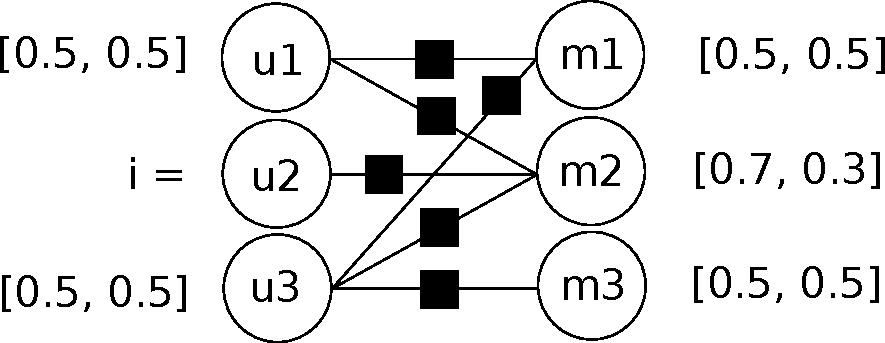
\includegraphics[scale=0.3]{graphics/top-n-graph.pdf}%
	      \caption{Factor Graph for predicting Top-N movies for user $\hat u = u_2$.
	      \label{top_n_graph}
	   }
	\end{subfigure}\hfill%
	\begin{subfigure}{.6\columnwidth}
	   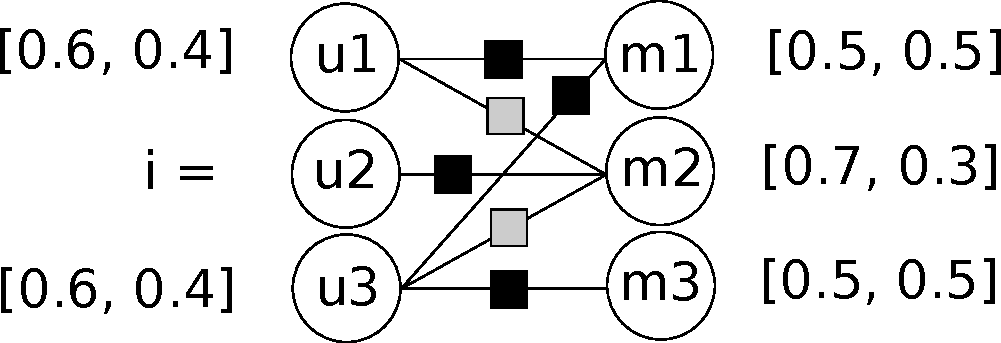
\includegraphics[scale=0.3]{graphics/top-n-important-messages.pdf}%
      	   \caption{Belief is propagated from observed node $m_2$ to unobserved nodes 
	      \label{top_n_graph_important_msg}
	   }
	\end{subfigure}\hfill%
	\begin{subfigure}{.6\columnwidth}
	   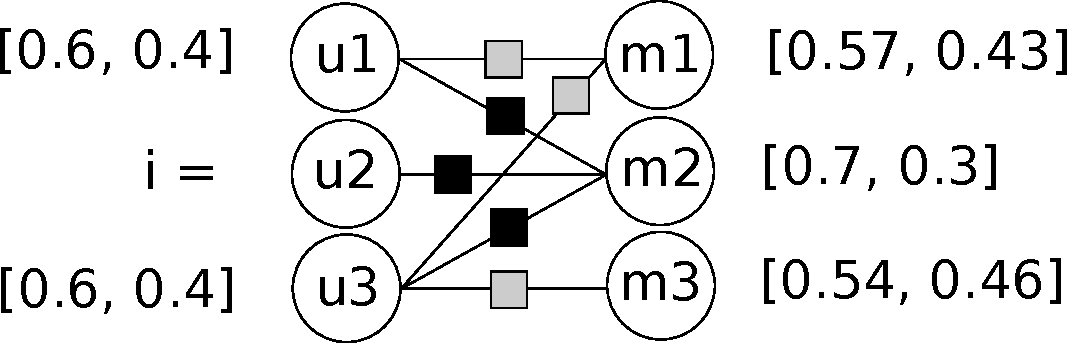
\includegraphics[scale=0.3]{graphics/top-n-final.pdf}%
	      \caption{A possible third state with $m_1$ being the top-1 recommendation for $u_2$. 
	      \label{top_n_graph_final_state}
	   }
	\end{subfigure}
	\caption{Top-N step by step}
\end{figure*}

\mypar{Cost Analysis}
A reasonable choice for the cost measure is the FLOP count, since BP operates on floating point numbers to calculate the beliefs. Unfortunately, it is not viable to calculate the exact amount of FLOPS for a given input size analytically, as BP is driven by the list of maximal message residuals and it cannot be foreseen, how many messages have to be calculated until convergence. Even worse, the count of processed messages (and, related, the FLOPS) is not only a function of the input \textit{size}, but also a function of the actual \textit{shape} of the graph. Therefore, we decided to count FLOPS using performance counters. The following counters were used:

\begin{itemize}
	\item FP\_COMP\_OPS\_EXE.SSE\_SCALAR\_SINGLE and \\FP\_COMP\_OPS\_EXE.SSE\_SCALAR\_DOUBLE:\\count the number of SSE instructions on single floats and doubles.
	\item FP\_COMP\_OPS\_EXE.SSE\_PACKED\_SINGLE and \\FP\_COMP\_OPS\_EXE.SSE\_PACKED\_DOUBLE:\\count the number of packed SSE instructions on floats and doubles.
	\item SIMD\_FP\_256.PACKED\_SINGLE and \\SIMD\_FP\_256.PACKED\_DOUBLE:\\count the number of packed AVX instructions on floats and doubles.
	\item FP\_COMP\_OPS\_EXE.X87:\\counts the legacy X87 floating point instructions.
\end{itemize}

The performance counters were evaluated using VTune Amplifier XE 2015 (see section~\ref{sec:results}).
Since it is impossible to distinguish the different kinds of operations, all FLOPS are weighted the same.


%\mypar{Discrete Fourier Transform}
%Precisely define the transform so I understand it even if I have never
%seen it before.
%
%\mypar{Fast Fourier Transforms}
%Explain the algorithm you use.
%
%\mypar{Cost Analysis}
%First define you cost measure (what you count) and then compute the
%cost. Ideally precisely, at least asymptotically. In the latter case you will need to instrument your code to count
%the operations so you can create a performance plot.
%
%Also state what is
%known about the complexity (asymptotic usually) 
%about your problem (including citations).